\chapter{Nix}

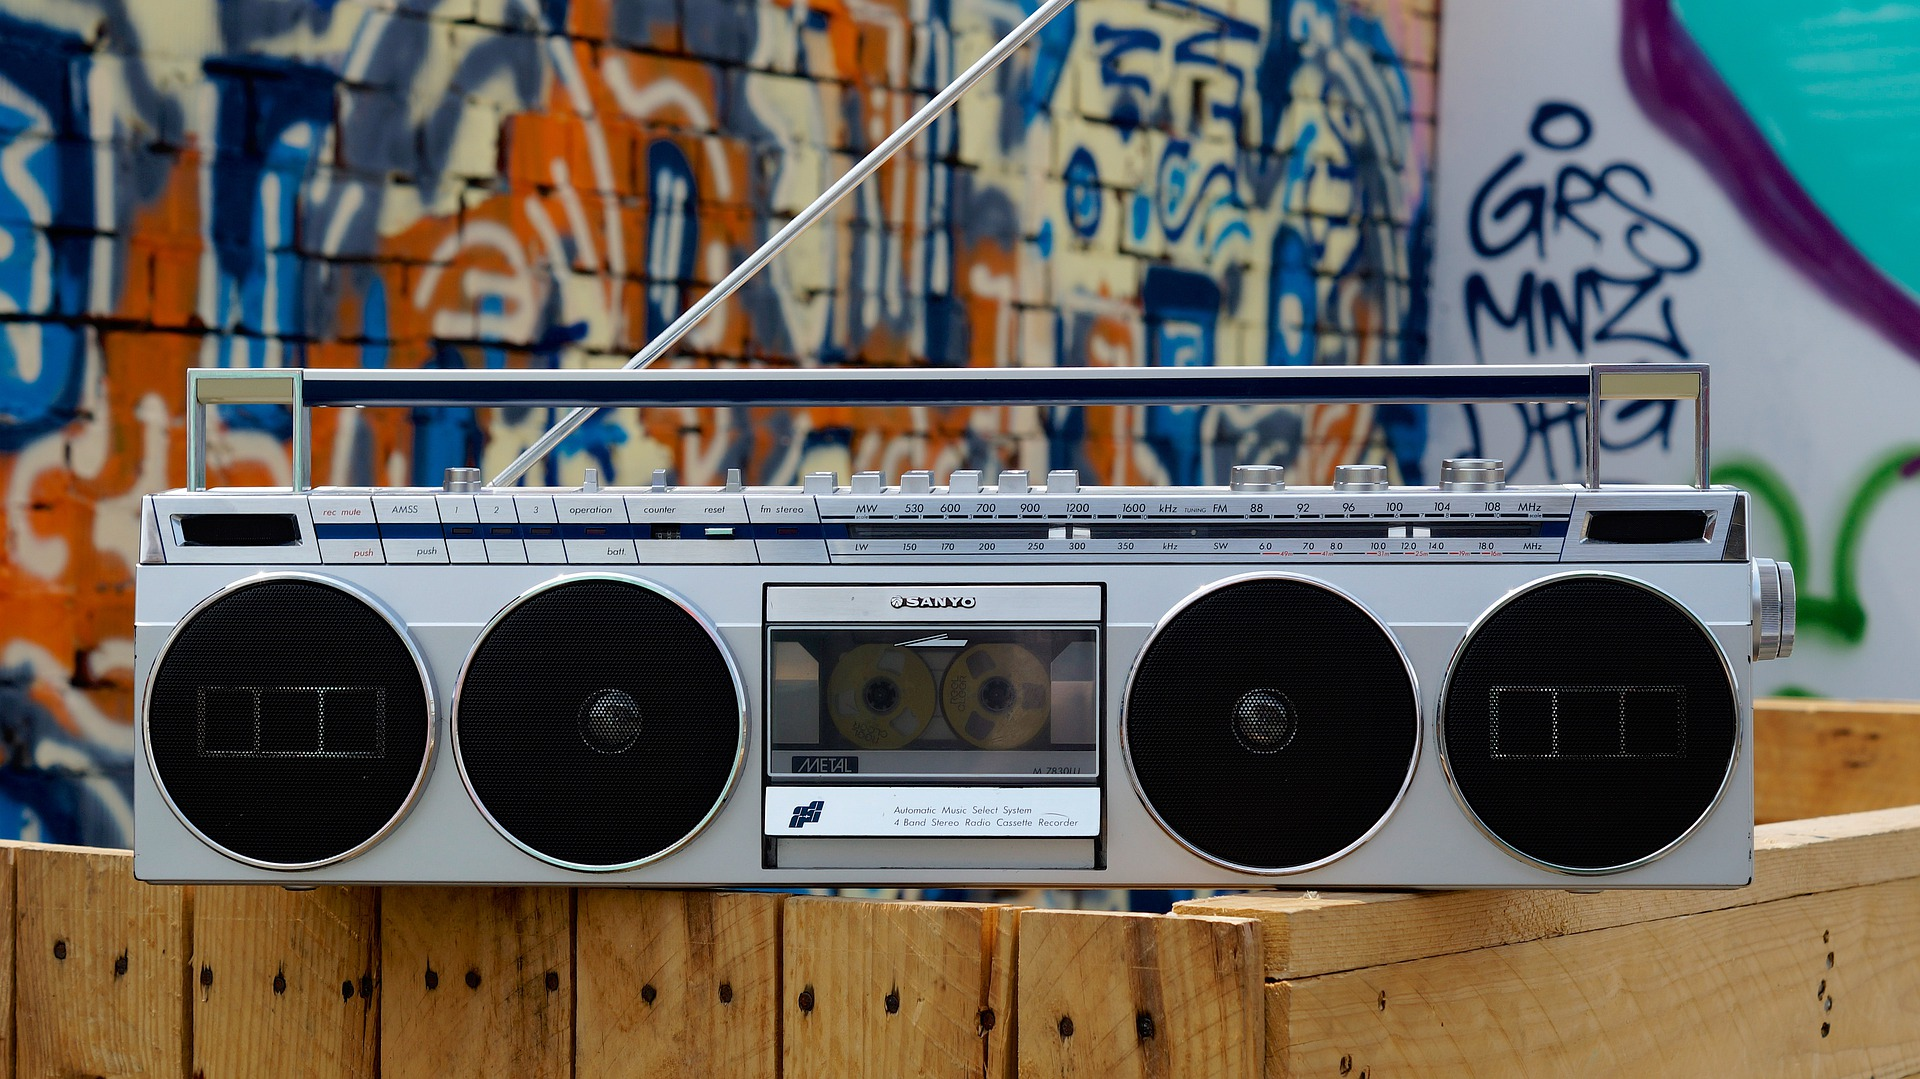
\includegraphics{25-nix.jpg}

\justifying
If you haven't tried Nix\index{Nix} yet, then now is a great time! The Nix ecosystem is all about
helping you reliably create ``nailed'' build environments. You as the developer get control over
the dependencies of a project, which increases  confidence in a high degree of fidelity around
expectations for your builds. Nix allows you to experiment in ways that don't break Nix itself,
or interfere with other projects on your system. Think ``virtualenv'' in Python,
but \href{https://github.com/NixOS/nixpkgs/tree/master/pkgs}{the nixpkgs repository}
allows you to mix and match support for multiple dependency version, languages, and more. There is a  \href{https://nixos.org/guides/how-nix-works.html}{well written introduction to Nix and how it works} available
on the web site for the project.

\justifying
Nix can be installed on your existing system, or used as a full operating system. For our purposes, we will
\href{https://nixos.org/download.html}{install nix to an existing environment} rather than go the full NixOs route.

\section{Setting up Nix as a Development Environment}

\justifying
In preparation for some labs using Nix, we will configure our development environment with nix-shell \href{https://nixos.wiki/wiki/Development_environment_with_nix-shell}{similar to the description at this web site}.

\section{Troubleshooting}

\justifying
Sometimes running nix-shell will fail with a ``Permission Denied'' error.

\begin{mybox}{\thetcbcounter: nix-shell error}
	\lstinputlisting{code/25-nix/nix-error.txt}
	\label{nixerr}
\end{mybox}

\justifying
To solve this error, you can type ``set -e NIX\_REMOTE'' in BASH shell.

\markdownInput{../labs/ch8/lab-8a.md}

\markdownInput{../labs/ch8/lab-8b.md}

\section{Nix Directory Structure}
\justifying
Files and folders relevant to the Nix portions of our project are shown in the diagram below.

\begin{figure}[!htb]
	\centering
	\chapter{Nix}

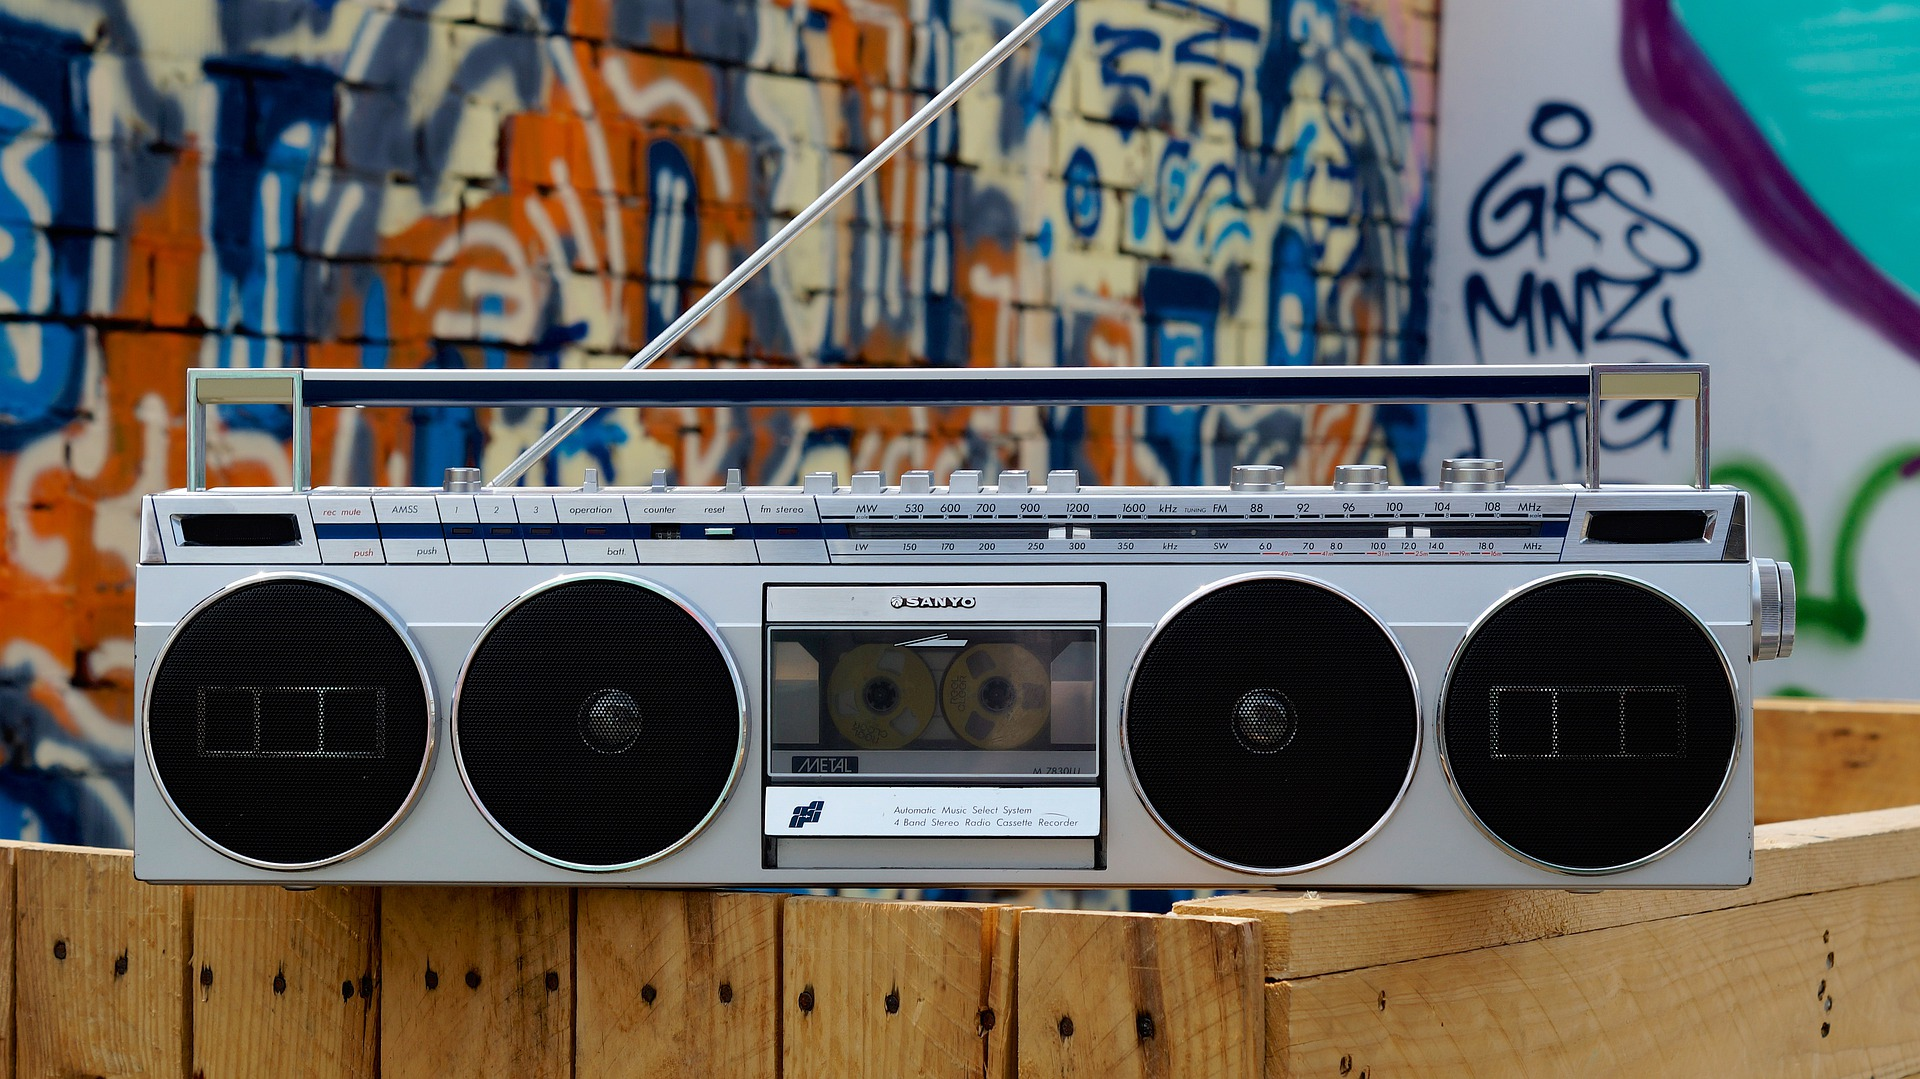
\includegraphics{25-nix.jpg}

\justifying
If you haven't tried Nix\index{Nix} yet, then now is a great time! The Nix ecosystem is all about
helping you reliably create ``nailed'' build environments. You as the developer get control over
the dependencies of a project, which increases  confidence in a high degree of fidelity around
expectations for your builds. Nix allows you to experiment in ways that don't break Nix itself,
or interfere with other projects on your system. Think ``virtualenv'' in Python,
but \href{https://github.com/NixOS/nixpkgs/tree/master/pkgs}{the nixpkgs repository}
allows you to mix and match support for multiple dependency version, languages, and more. There is a  \href{https://nixos.org/guides/how-nix-works.html}{well written introduction to Nix and how it works} available
on the web site for the project.

\justifying
Nix can be installed on your existing system, or used as a full operating system. For our purposes, we will
\href{https://nixos.org/download.html}{install nix to an existing environment} rather than go the full NixOs route.

\section{Setting up Nix as a Development Environment}

\justifying
In preparation for some labs using Nix, we will configure our development environment with nix-shell \href{https://nixos.wiki/wiki/Development_environment_with_nix-shell}{similar to the description at this web site}.

\section{Troubleshooting}

\justifying
Sometimes running nix-shell will fail with a ``Permission Denied'' error.

\begin{mybox}{\thetcbcounter: nix-shell error}
	\lstinputlisting{code/25-nix/nix-error.txt}
	\label{nixerr}
\end{mybox}

\justifying
To solve this error, you can type ``set -e NIX\_REMOTE'' in BASH shell.

\markdownInput{../labs/ch8/lab-8a.md}

\markdownInput{../labs/ch8/lab-8b.md}

\section{Nix Directory Structure}
\justifying
Files and folders relevant to the Nix portions of our project are shown in the diagram below.

\begin{figure}[!htb]
	\centering
	\chapter{Nix}

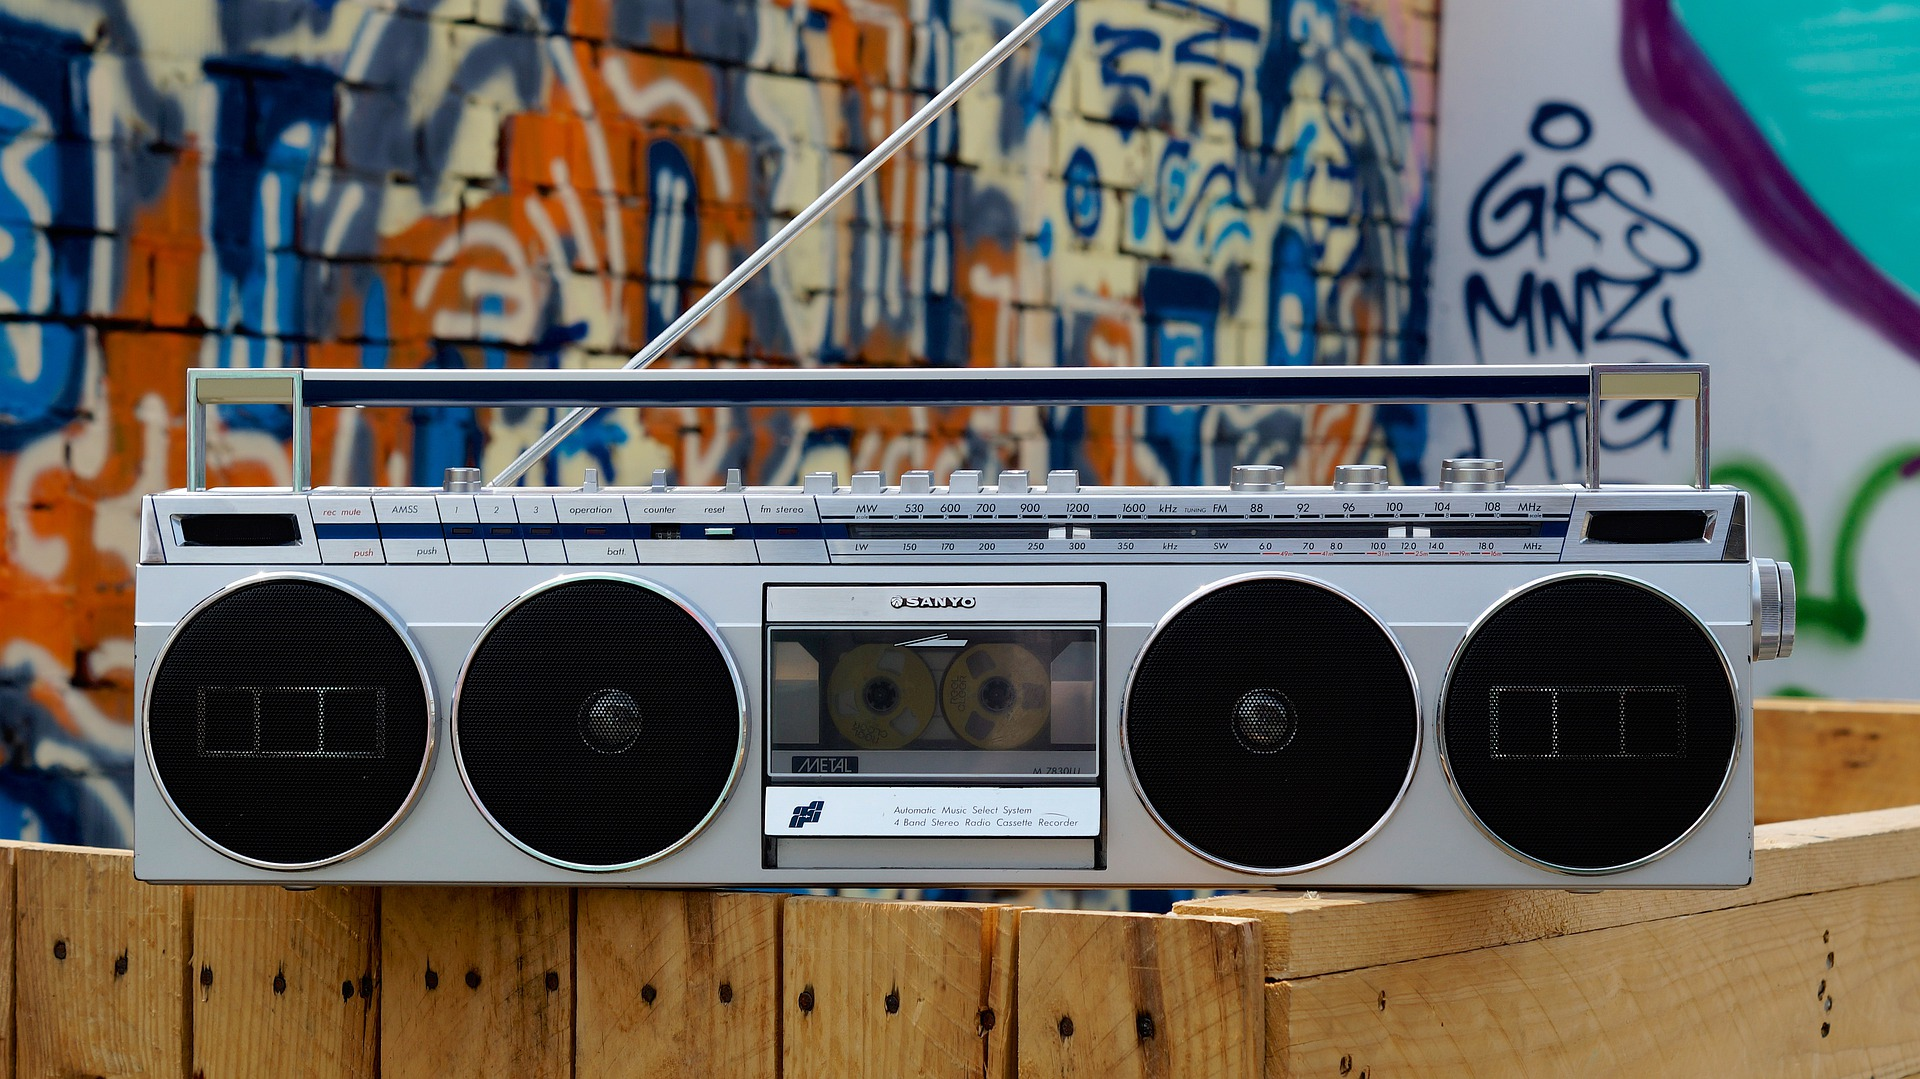
\includegraphics{25-nix.jpg}

\justifying
If you haven't tried Nix\index{Nix} yet, then now is a great time! The Nix ecosystem is all about
helping you reliably create ``nailed'' build environments. You as the developer get control over
the dependencies of a project, which increases  confidence in a high degree of fidelity around
expectations for your builds. Nix allows you to experiment in ways that don't break Nix itself,
or interfere with other projects on your system. Think ``virtualenv'' in Python,
but \href{https://github.com/NixOS/nixpkgs/tree/master/pkgs}{the nixpkgs repository}
allows you to mix and match support for multiple dependency version, languages, and more. There is a  \href{https://nixos.org/guides/how-nix-works.html}{well written introduction to Nix and how it works} available
on the web site for the project.

\justifying
Nix can be installed on your existing system, or used as a full operating system. For our purposes, we will
\href{https://nixos.org/download.html}{install nix to an existing environment} rather than go the full NixOs route.

\section{Setting up Nix as a Development Environment}

\justifying
In preparation for some labs using Nix, we will configure our development environment with nix-shell \href{https://nixos.wiki/wiki/Development_environment_with_nix-shell}{similar to the description at this web site}.

\section{Troubleshooting}

\justifying
Sometimes running nix-shell will fail with a ``Permission Denied'' error.

\begin{mybox}{\thetcbcounter: nix-shell error}
	\lstinputlisting{code/25-nix/nix-error.txt}
	\label{nixerr}
\end{mybox}

\justifying
To solve this error, you can type ``set -e NIX\_REMOTE'' in BASH shell.

\markdownInput{../labs/ch8/lab-8a.md}

\markdownInput{../labs/ch8/lab-8b.md}

\section{Nix Directory Structure}
\justifying
Files and folders relevant to the Nix portions of our project are shown in the diagram below.

\begin{figure}[!htb]
	\centering
	\chapter{Nix}

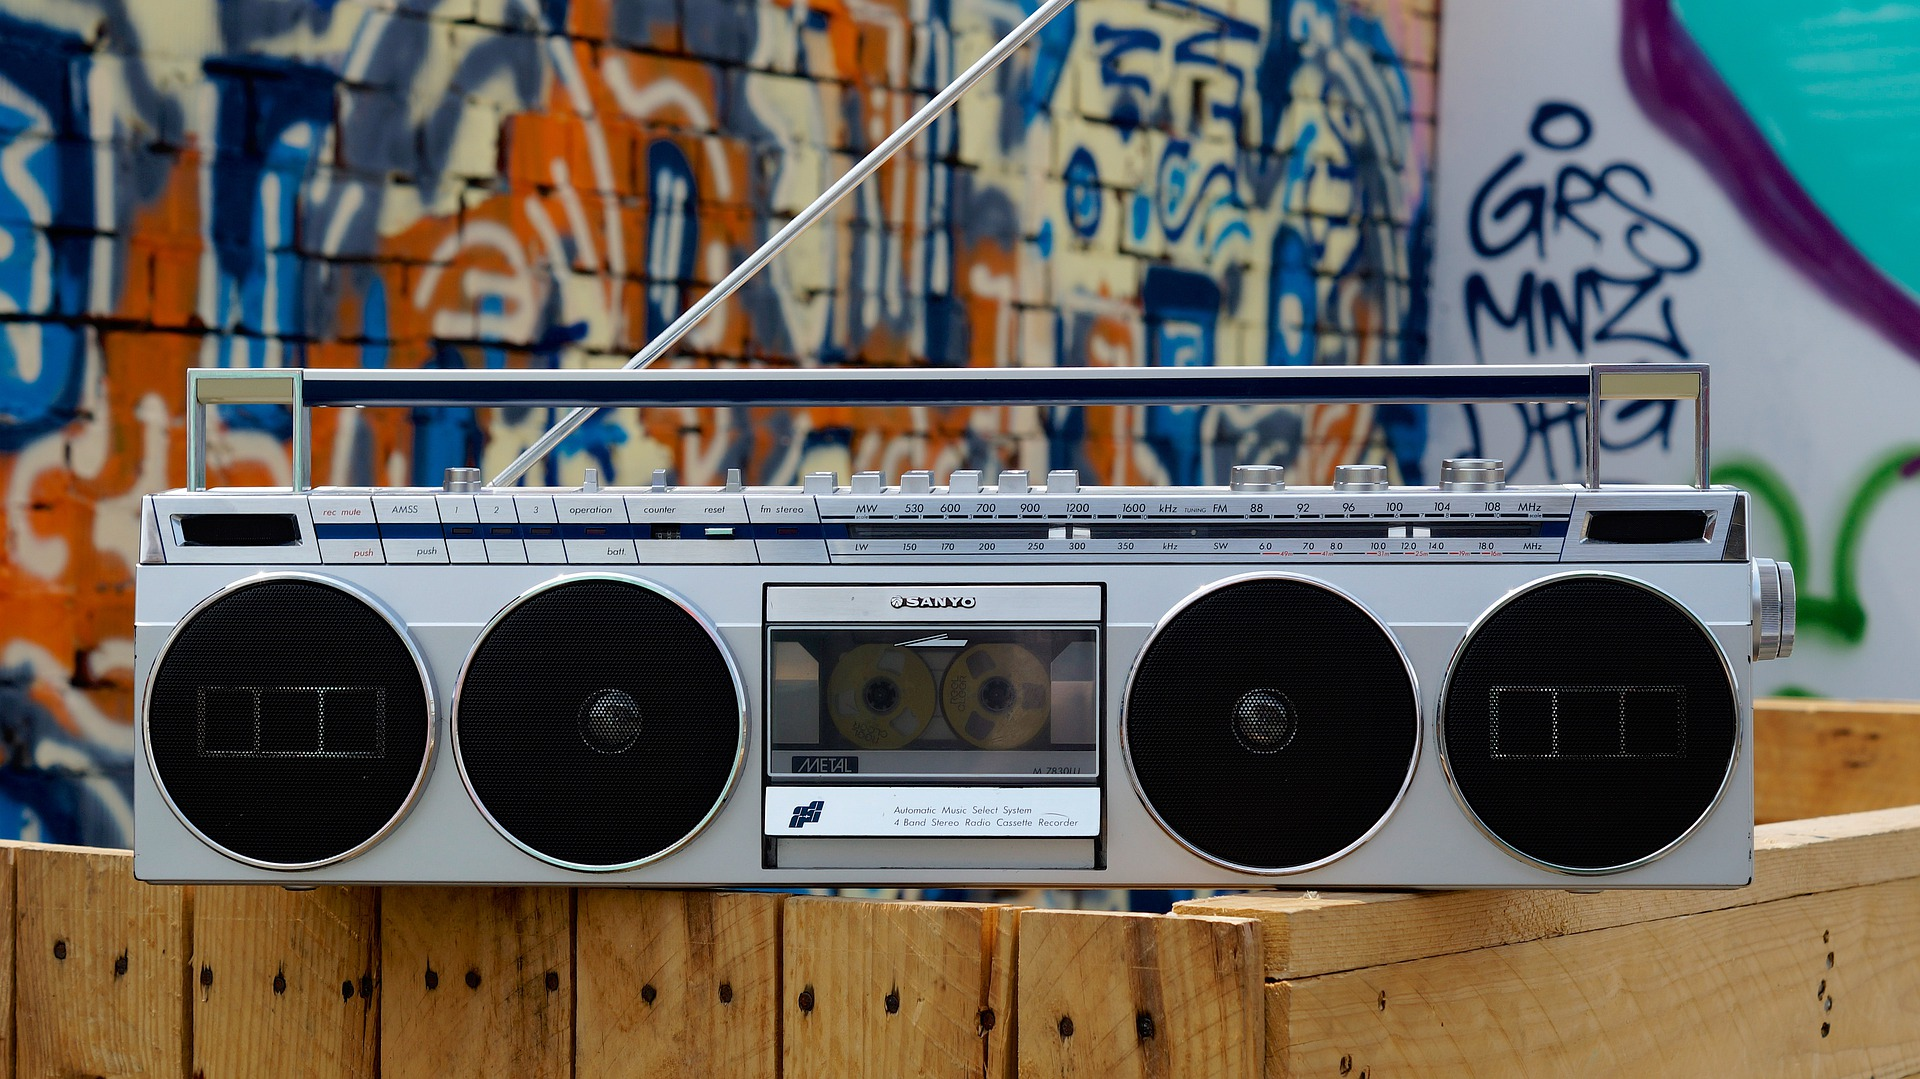
\includegraphics{25-nix.jpg}

\justifying
If you haven't tried Nix\index{Nix} yet, then now is a great time! The Nix ecosystem is all about
helping you reliably create ``nailed'' build environments. You as the developer get control over
the dependencies of a project, which increases  confidence in a high degree of fidelity around
expectations for your builds. Nix allows you to experiment in ways that don't break Nix itself,
or interfere with other projects on your system. Think ``virtualenv'' in Python,
but \href{https://github.com/NixOS/nixpkgs/tree/master/pkgs}{the nixpkgs repository}
allows you to mix and match support for multiple dependency version, languages, and more. There is a  \href{https://nixos.org/guides/how-nix-works.html}{well written introduction to Nix and how it works} available
on the web site for the project.

\justifying
Nix can be installed on your existing system, or used as a full operating system. For our purposes, we will
\href{https://nixos.org/download.html}{install nix to an existing environment} rather than go the full NixOs route.

\section{Setting up Nix as a Development Environment}

\justifying
In preparation for some labs using Nix, we will configure our development environment with nix-shell \href{https://nixos.wiki/wiki/Development_environment_with_nix-shell}{similar to the description at this web site}.

\section{Troubleshooting}

\justifying
Sometimes running nix-shell will fail with a ``Permission Denied'' error.

\begin{mybox}{\thetcbcounter: nix-shell error}
	\lstinputlisting{code/25-nix/nix-error.txt}
	\label{nixerr}
\end{mybox}

\justifying
To solve this error, you can type ``set -e NIX\_REMOTE'' in BASH shell.

\markdownInput{../labs/ch8/lab-8a.md}

\markdownInput{../labs/ch8/lab-8b.md}

\section{Nix Directory Structure}
\justifying
Files and folders relevant to the Nix portions of our project are shown in the diagram below.

\begin{figure}[!htb]
	\centering
	\input{dot/25-nix.tex}
	\caption{Nix directory and related files.}
	\label{nixfiles}
\end{figure}

	\caption{Nix directory and related files.}
	\label{nixfiles}
\end{figure}

	\caption{Nix directory and related files.}
	\label{nixfiles}
\end{figure}

	\caption{Nix directory and related files.}
	\label{nixfiles}
\end{figure}
